


\chapter{Measures of distance}
\label{dist}

We take a little time out here to consider some ideas regarding multivariate distance and introduce some properties of multivariate distance matrices.   These concepts are most obviously relevant when considering multivariate technique such as cluster analysis and scaling methods, where we wish to examine the difference between individuals.   In doing this, we need to find some definition of the concept of ``difference between individuals'', and will therefore consider a range of proximity measures.   We also provide some discussion of difference between variables.   These are currently important concepts in bio-informatic applications but earlier work in multivariate statistics involved consideration of variables which may be carrying similar information where cluster analysis of variables could be used as a preliminary data analytical exercise.   We start by considering one particular measure, the Mahalanobis distance.

\section{Mahalanobis Distance}
\label{standarddist}

The Mahalanobis distance has an important role in multivariate theory, albeit this is often an implied consideration rather than an explicit one.   For example, development of forms of discriminant analysis considered in chapter \ref{discriminant} involve this measure.   There are however a number of important distributional properties of the Mahalanobis distance which could be more used in determining multivariate normality.    It should be noted that use of standard distance requires a parametric view of the world, and in particular it is most applicable for symmetric distributions.   We follow \cite{Flury:1997} in providing the following exposition of the standard distance.  

Firstly, if we consider the \emph{univariate} standard distance we see that this is a measure of the absolute distance between two observations in units of their standard deviation.
\marginnote{The standardisation is important; this measure it is invariant under non-degenerate linear transformations.   A univariate example would be given by considering $Y = \alpha  + \beta X$, where $\beta \neq 0$ and $\alpha$ are fixed constants.   Consider transforming $x_{1}$ and $x_{2}$ to $y_{i} = \alpha + \beta x_{i}; i = 1,2$. Then considering the standard distance between these two transformed variables we find:

\begin{eqnarray*}
d(y_{1},y_{2}) &=& \frac{|y_{1} - y_{2}|}{\sqrt{var(Y)}}\\
 &=&  \frac{|\beta(x_{1} - x_{2}|)}{\sqrt{\beta^{2}\sigma^{2}}}\\
 &=& d(x_{1},x_{2})
\end{eqnarray*}
}
Given $X$, a random variable with mean $\mu$ and variance $\sigma^{2} > 0$, the \emph{standard distance}, between two numbers $x_{1}$ and $x_{2}$ is defined as follows:

\begin{displaymath}
d(x_{1}, x_{2}) = \frac{|x_{1} - x_{2}|}{\sigma}
\end{displaymath}

\marginnote{Where $\sigma = 1$, this standard distance is the same as the Euclidean distance given later in section \ref{euclidean}}.

The univariate standard distance has a straightforward generalisation to a multivariate setting.   Considering now two vectors  $\boldsymbol{x}_{1}$ and $\boldsymbol{x}_{2}$, with a common covariance matrix $\boldsymbol{\Sigma}$ the multivariate standard distance is given by:

\begin{displaymath}
d(\boldsymbol{x}_{1},\boldsymbol{x}_{2}) = \sqrt{(\boldsymbol{x}_{1} - \boldsymbol{x}_{2})^{T}\boldsymbol{\Sigma}^{-1}(\boldsymbol{x}_{1},\boldsymbol{x}_{2}) }
\end{displaymath}

Depending on whichever textbook is consulted, this multivariate standard distance may be referred to as the \emph{statistical distance}, the \emph{elliptical distance} or the \emph{Mahalanobis distance}.   \cite{Flury:1997} notes that the squared Mahalanobis distance $d(\boldsymbol{x}_{1},\boldsymbol{x}_{2})^{2}$ is sometimes simply referred to as the Mahalanobis distance, although it is not a valid distance measure.   We refer here to the multivariate standard distance,  $d(\boldsymbol{x}_{1},\boldsymbol{x}_{2})$ as the Mahalanobis distance, and where necessary, to  $d(\boldsymbol{x}_{1},\boldsymbol{x}_{2})^{2}$ as the \emph{squared} Mahalanobis distance.


It is worth noting that this measure was originally proposed by
\cite{Mahalanobis:1930} as a measure of distance between two populations:

\begin{displaymath}
\Delta(\boldsymbol{\mu}_{1},\boldsymbol{\mu}_{2}) = \sqrt{(\boldsymbol{\mu}_{1} - \boldsymbol{\mu}_{2})^{T}\boldsymbol{\Sigma}^{-1}(\boldsymbol{\mu}_{1},\boldsymbol{\mu}_{2}) }
\end{displaymath}
which has an obvious sample analogue as the distance between two mean vectors:

\begin{displaymath}
\Delta(\boldsymbol{\bar{x}}_{1},\boldsymbol{\bar{x}}_{2}) = \sqrt{(\boldsymbol{\bar{x}}_{1} - \boldsymbol{\bar{x}}_{2})^{T}\boldsymbol{S}^{-1}(\boldsymbol{\bar{x}}_{1},\boldsymbol{\bar{x}}_{2}) }
\end{displaymath}
where $\boldsymbol{S}$ is the pooled estimate of $\boldsymbol{\Sigma}$ given by $\boldsymbol{S} = \left[ (n_{1}-1) \boldsymbol{S}_{1} +  (n_{2}-1) \boldsymbol{S}_{2} \right] / (n_{1} + n_{2} - 2)$.

Here, we are going to consider the distance between $\boldsymbol{x}$, a vector of random variables with mean $\boldsymbol{\mu}$ and covariance matrix $\boldsymbol{\Sigma}$ and its mean:

\begin{displaymath}
\Delta(\boldsymbol{x},\boldsymbol{\mu}) = \sqrt{(\boldsymbol{x} - \boldsymbol{\mu})^{T}\boldsymbol{\Sigma}^{-1}(\boldsymbol{x},\boldsymbol{\mu}) }
\end{displaymath}
and clearly we can find a sample analogue by estimating $\boldsymbol{\mu}$ by $\hat{\boldsymbol{x}}$ and $\boldsymbol{\Sigma}$ by $\boldsymbol{S} = \frac{1}{n-1} \boldsymbol{X}^{T}\boldsymbol{X}$.  We note that in \textbf{R}, the \verb+mahalanobis()+ function is intended to returns the \emph{squared} multivariate distance between a matrix $\boldsymbol{X}$ and a mean vector $\boldsymbol{\mu}$, given a user-supplied covariance matrix $\boldsymbol{\Sigma}$, i.e. we wish to calculate: 

\begin{displaymath}
d(\boldsymbol{x}_{i},\hat{\boldsymbol{\mu}})^{2} 
= (\boldsymbol{x}_{i} - \hat{\boldsymbol{\mu}})^{T}
\hat{\boldsymbol{\Sigma}}^{-1}
(\boldsymbol{x}_{i} - \hat{\boldsymbol{\mu}}) 
\end{displaymath}

We could also consider the Mahalanobis angle $\theta$ between two vectors at the origin:

\begin{displaymath}
\cos \theta = \frac{\boldsymbol{x}_{1}^{T} \boldsymbol{S}^{-1} \boldsymbol{x}_{2}}
{d(\boldsymbol{x}_{1},\boldsymbol{0})d(\boldsymbol{x}_{2},\boldsymbol{0})}
\end{displaymath}

This can be extracted from within $\boldsymbol{R}$ using the following:

\begin{Schunk}
\begin{Sinput}
> mahangle <- function(x1, x2, covmat){
+   zero <- vector("numeric", length(x1) )  
+   num <- t(x1) %*% solve(covmat) %*% x2
+   denom <- sqrt(mahalanobis(x1, zero, covmat)) * 
+      sqrt(mahalanobis(x2, zero, covmat)) 
+   angle <- acos(num / denom)
+   return(angle)
+ }
\end{Sinput}
\end{Schunk}

\subsection{Distributional properties of the Mahalanobis distance}

Remembering that where $z_{1}, \ldots, z_{p} \sim N(0,1)$, if we form $y = \sum_{j=1}^{p} z_{j}^{2}$ then $y \sim \chi_{p}^{2}$ \citep{Bilodeau+Brenner:1999}; for multivariate normal data, with $p$ variables, the squared Mahalanobis distance can be considered against a $\chi_{p}^{2}$ distribution:

\begin{equation}
(\boldsymbol{x}_{i} - \hat{\boldsymbol{\mu}})^{T}
\hat{\boldsymbol{\Sigma}}^{-1}
(\boldsymbol{x}_{i} - \hat{\boldsymbol{\mu}}) = \boldsymbol{z}^{T}\boldsymbol{z} \sim \chi^{2}_{p}
\end{equation}

This immediately affords one method for assessing multivariate normality, quantiles of the Mahalanobis distance of $\boldsymbol{x}_{i}$, $i = 1, \ldots, n$ with respect to $\boldsymbol{\mu}$ can be plotted against quantiles of the $\chi^{2}_{p}$ distribution as an assessment of multivariate normality.

\begin{figure}
\begin{center}
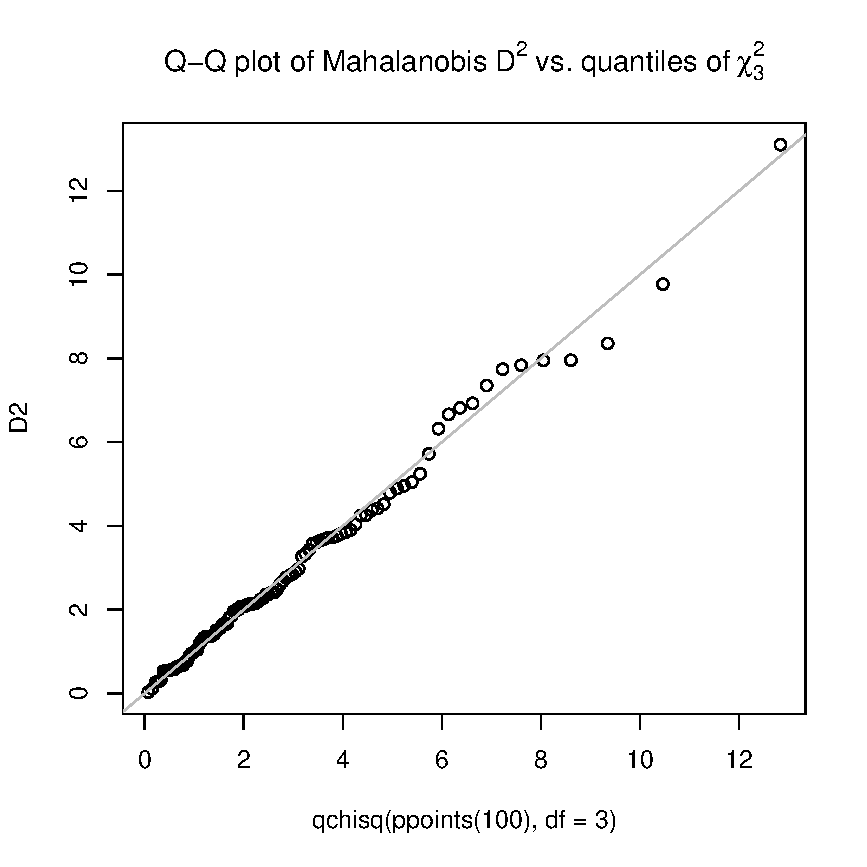
\includegraphics[width = 0.5\textwidth]{images/DistChiPlot}
\caption{QQ plot of squared Mahalahobis distance plotted against $\chi^{2}$ distribution}
\label{qqchimahlanobis}
\end{center}
\end{figure}

We can also define contours as a set of points of equal probility in terms of equal Mahalanobis distance:

\begin{equation}
(\boldsymbol{x}_{i} - \hat{\boldsymbol{\mu}})^{T}
\hat{\boldsymbol{\Sigma}}^{-1}
(\boldsymbol{x}_{i} - \hat{\boldsymbol{\mu}}) = \boldsymbol{z}^{T}\boldsymbol{z} = c^{2}
\end{equation}

for any constant $c > 0$.  We will also find later in section \ref{mahalpca} that the squared Mahalanobis distance is equivalent to the sum of squared prinicipal component scores.   However, this chapter on distance is implicitly geared towards presentations in the chapter \ref{clustan} on cluster analysis as well as  chapter \ref{mds} on scaling methods.   In that context it is worth noting that Mahalanobis distance is rarely used in cluster analysis, certainly \cite{Kendall:1975} points out its limitations in this context.  Sporadic reports in the literature include \cite{Maronna+Jacovkis:1974} who report use of a particular clustering algorithm, $k$-means, with the Mahalanobis distance whereas \cite{Gnanadesikan+etal:1993} use it with hierarchical cluster analysis.   This latter work may illustrate one of the difficulties in using the Mahalanobis distance in the requirement to assume a common covariance.     However, whilst not proposing it's use in an automatic clustering algorithm, \cite{Atkinson+etal:2004} report use of Mahalanobis distance within the forward search to reliably identify subgroups within the data.   They propose a small modification to the Mahalanobis distance for use in cluster analysis as follows.   The Mahalanobis distance is multiplied by $(|\hat{\boldsymbol{\Sigma}}^{-1}_{k}|^{1/2})^{r}$ for group $k$.   Where $r=0$ we have the usual distance, when $r=1$ we have what they call the \emph{standardised} Mahalanobis distance which eliminates the different variance between groups.

Having provided an overview of one distributionally important distance measure, before considering further measures we consider a few definitions.   \cite{Flury:1997} notes that the squared Mahalanobis distance does not satisfy the axioms of distance.

\section{Definitions}
\label{distdefinitions}

We now formalise our idea of a proximity measure.  This term encapsulates both similarity and disssimilarity measures which have the obvious interpretation (measuring similarity and dissimilarity between entities), and can be found from each other by means of an appropriate monotonic transformation.   We usually assume that these measures are symmetic.

A \emph{distance} can be defined as a function $d(\cdot)$ that satisfies the following properties:

\begin{itemize}
\item[(1)] Non-negative, that is $d(\boldsymbol{x},\boldsymbol{y}) \geq 0$ for all $\boldsymbol{x},\boldsymbol{y} \in \mathbb{R}^{p}$ and 
\item[(2)] Identified, that is $d(\boldsymbol{x},\boldsymbol{x}) = 0$ for all $\boldsymbol{x} \in \mathbb{R}^{p}$;
\item[(3)] Symmetric, that is $d(\boldsymbol{x},\boldsymbol{y}) = d(\boldsymbol{y},\boldsymbol{x})$ for all $\boldsymbol{x},\boldsymbol{y} \in \mathbb{R}$;
\end{itemize}

In addition to satisfying these three properties, a \emph{metric} also satisfies the following two properties:
\begin{itemize}
\item[(4)] Definite, that is $d(\boldsymbol{x},\boldsymbol{y}) = 0$ if and only if $\boldsymbol{x} = \boldsymbol{y}$ for all $\boldsymbol{x},\boldsymbol{y} \in \mathbb{R}^{p}$;
\item[(5)] Triange inequality $d(\boldsymbol{x},\boldsymbol{y}) + d(\boldsymbol{y},\boldsymbol{z}) \geq d(\boldsymbol{x},\boldsymbol{z})$ for all $\boldsymbol{x},\boldsymbol{y},\boldsymbol{z} \in \mathbb{R}$  
\end{itemize}


It is worth noting that it is possible to compute a similarity measure, often denoted $s$, where $0 \leq S \leq 1$.   A \emph{similarity} function $s(\cdot,\cdot)$ satisfies (1) non-negativity $s(\boldsymbol{x}, \boldsymbol{y}) \geq 0$, (2) symmetry $S(\boldsymbol{x},\boldsymbol{y}) = s(\boldsymbol{y},\boldsymbol{x})$ as well as:

\begin{itemize}
\item[(3)] $s(\boldsymbol{x}, \boldsymbol{y})$ increases in a monotone fashion as $\boldsymbol{x}$ and $\boldsymbol{y}$ become more similar.   A \emph{dissimilarity} function satisfies the first two but clearly 3 is reversed, i.e. it decreases as  $\boldsymbol{x}$ and $\boldsymbol{y}$ become more similar.  
\end{itemize}

Dissimilarity is the opposite of similarity, therefore any monotonically decreasing transformation of $s$ can provide a dissimilarity measure.   The most obvious tranform would be to take $d = 1 - s$ but we will consider a few alternatives later.

\section{Distance between points}
\label{pointdistance}

Two \textbf{R} packages are needed to provide most of the distance functions considered here.   In addition to the default \verb+stats+ library, which provides the \verb+dist()+ function, we require the \verb+cluster+ package for the \verb+daisy()+ function.   Some further correlation based measures can be found in the \verb+Dist()+ function in the \verb+amap+ package as well as \verb+BioBase+ from Bioconductor.

We now consider a range of ways in which a multivariate distance can be measured.  In conducting an analysis, some decision needs to be made as to whether to scale variables, or whether to remove highly correlated variables from the analysis.   For example, \cite{Gnanadesikan:1997} gives an artificial example which illustrates how rescaling variables can subsequently alter impression of groupings.


\subsection{Quantitative variables - Interval scaled}
\label{distancequant}

It is reasonably straightforward to suggest a number of dissmilarity measures $d_{ij}$ which measure the distance between individual $i$ and $j$.

%\begin{itemize}
%\item 
\subsection{Euclidean distance}.
\label{euclidean}

The Euclidean distance, or the $l_{2}$ norm, is perhaps the most commonly used distance measure.   As mentioned in section \ref{standarddist}, this distance could be considered simply as the Mahalanobis distance where $\sigma$ = 1.   Especially in the context of cluster analysis, where we hope to identify distinct sub-groups within the data, it is not clear how we might determine the covariance matrix hence the Mahalanobis distance has seen little use.   The Euclidean distance, which is quite simply the square root of the squared distance between any two vectors, which can be quite simply interpreted as the physical distance between two $p$-dimensional points is also a convenient measure to understand.  Formally, we can express this measure as:

\begin{displaymath}
\label{euclideanF}
d_{ij} =  \left( \Sigma_{k=1}^{p} (x_{ik} - x_{jk})^2 \right)^{\frac{1}{2}}
\end{displaymath}

where we are trying to measure the distance between observations in row $i$ and row $j$, in other words $x_{ik}$ is the $k$th observation in row $i$, and $x_{jk}$ is the corresponding $k$th observation in row $j$.   Euclidean distance can be readily calculated in \textbf{R} using the \verb+dist()+ function with the default \verb+method = "euclidean"+, as well as by \verb+daisy()+ with the default \verb+metric = "euclidean"+, although in \verb+daisy()+ it is possible to standardise the data within the calculations by adding \verb+stand = TRUE+ to the function call.
 

\subsection{Scaled Euclidean distance}
\label{scaledeuclidean}

It is possible to introduce a suitable weight $w_{k}$ such as the inverse of the standard deviation of the $k$th variable, i.e. $w_{k} = s_{k}^{-1}$, or even the inverse of the range of the data.

\begin{displaymath}
\label{scaledeuclideanF}
d_{ij} = \sqrt{\left( \Sigma_{k=1}^{p} w_{k}^{2}(x_{ik} - x_{jk})^2 \right)}
\end{displaymath}

No explicit routines are available to compute this measure, but clearly if the co-ordinates are rescaled by $\sqrt{w_{k}}$ this can be calculated implicitly.

\subsection{City Block metric}
\label{cityblock}

The City Block metric, formally referred to as an $l_{1}$ norm, measures the absolute difference between two vectors.   It is so-named because it measures the distance between two points in terms of movements parallel to the axis and therefore resembles the distance between two points in a city.   \cite{Krause:1975} (who had obviously never been in a London taxi) called this distance the \emph{taxicab} distance, \cite{Brandeau+Chiu:1988} used the term \emph{rectilinear}, but perhaps the most common alternative name is \emph{Manhattan}, suggested by \cite{Larson+Sadiq:1983} reflecting the famous city block layout in Manhattan.   Formally, we can express this distance as:

\begin{displaymath}
\label{cityblockF}
d_{ij} =  \left( \Sigma_{k=1}^{p} |x_{ik} - x_{jk}| \right)
\end{displaymath}

It can be calculated in R using the \verb+dist()+ function with \verb+method = "manhattan"+



\subsection{Minkowski metric}
\label{minkowski}

The Minkowski metric, or the $l_{r}$ norm, is a generalisation of the Manhattan and Euclidean distances.

\begin{displaymath}
\label{minkowskiF}
d_{ij} =  \left( \Sigma_{k=1}^{p} |x_{ik} - x_{jk}|^\lambda \right)^{1/\lambda}
\end{displaymath}

Where $\lambda = 1$ we have the Manhattan metric, where $\lambda = 2$ we have the Euclidean distance.   It can be noted that increasing $\lambda$ exaggerates dissimilar units relative to similar ones.   This metric can be calculated in R using the \verb+dist()+ function with \verb+method = "minkowski"+ but additionally requires an argument to \verb+p+ to set $\lambda$, the power of this distance.   Therefore, for example \verb+dist(x, method = "minkowski", p=2)+ gives the Euclidean distance for matrix \verb+x+. 

\subsection{Canberra metric}
\label{canberra}

The Canberra metric \citep{Lance+Williams:1966} can be regarded as a generalisation of binary dissimilarity measures, and is very sensitive to small changes close to $x_{ik} = x_{jk} = 0$.   It can be scaled by division by $p$, the number of variables to ensure it lies in the range (0,1).   Terms with zero numerator and denominator are omitted from the sum and treated as if the values were missing.

\begin{displaymath}
\label{canberraF}
d_{ij} = \left\{ \begin{array}{ll} 0 & for\ x_{ik} = x_{jk} = 0\\
  \Sigma\left( \frac{|x_{ik} - x_{jk}|}{ |x_{ik} + x_{jk}|} \right) & for\  x_{ik} \neq 0\ or\  x_{jk} \neq 0 \end{array} \right.
\end{displaymath}

This metric can be calculated in \textbf{R} using the \verb+dist()+ function with \verb+method = "canberra"+

\subsection{Czekanowski Coefficient}
\label{czekanowski}

Finally, we mention the Czekanowski Coefficient, which for continuous variables can be given as:

\begin{displaymath}
\label{czekanowskiF}
d_{ij} = 1 - \frac{2 \sum_{k=1}^{p} min(x_{ik},x_{jk})}{\sum_{k=1}^{p}(x_{ik} + x_{jk})}
\end{displaymath}

%\end{itemize}


\subsection{Distance between variables}
\label{corrdist}

We next consider a number of correlation based distance measures.   Note that when used conventionally for calculating the correlation between two variables we work with standardised columns.  In order to measure the similarity between two individuals we must therefore work with standardised rows, this may not be a sensible procedure.   For example, if variables are measured on different scales the idea of a row mean may not be clear.   There is further material in the literature questioning the use of these measures \citep{Jardine+Sibson:1971,Fleiss+Zubin:1969} and \cite{Everitt+etal:2001} note that correlation measures cannot distinguish the size of two different observations, giving the example $\boldsymbol{x}^{T}_{1} = c(1,2,3)$ and $\boldsymbol{x}^{T}_{2} = c(1,2,3)$ have correlation $\rho_{12} = 1$ yet $\boldsymbol{x}^{T}_{2}$ is three times the size of $\boldsymbol{x}^{T}_{1}$.   Nevertheless, correlation based measures have become particular popular in a bio-informatics setting where some of the noted limitations do not apply (all variables are measured on a comparable scale) and in fact it is not always clear what a row and a column mean in that application area.   

We therefore consider four four distances that can be obtained a correlation measure.  Some thought needs to be given to determining the transformation from a correlation coefficient to a distance measure.   The Pearson correlation coefficient is defined in the range $-1 \leq \rho_{ij} \leq 1$.   \cite{Everitt+etal:2001} suggest using $d_{ij} = \frac{1 - \rho_{ij}}{2}$.  \cite{Gentleman+etal:2005} suggest that it may be appropriate under some circumstances to use the absolute value of the correlation, that is $d_{ij} = 1 - |\rho_{ij}|$ which means that there will be little distance between rows having strong positive and strong negative correlation.   In terms of measuring the dissimilarity between variables, \cite{Krzanowski:2000} suggests a further alternative using  $d_{ij} = 1 - (\rho_{ij})^{2}$.   Examining pre-Bioinformatics data, \cite{Lance+Williams:1979} who compared a number of transformations and expressed a strong preference for the first transformation, and a strong disdain for the third.

It should be noted that these measures are quite badly affected by outliers.   As a result, non-parametric versions may often be preferred.   Conversely, these measures are invariant to change of location or scale transformation which is rather useful.   It should be noted in bio-informatics practice that they tend to group genes whose expression patterns are linearly related, there is some empirical support from that application for their use in a particular context.

\subsection{Pearson correlation distance}
\label{pearsondist}

\begin{displaymath}
\label{pearsondistF}
d(x_{ij},x_{ik}) = 1 - \rho_{ij} = 1 - \frac{\sum_{i=1}^{p} (x_{ij} - \bar{x}_{\cdot j}) (x_{ik} - \bar{x}_{\cdot k}}{\sqrt{\sum_{i=1}^{p} (x_{ij} - \bar{x}_{\cdot j})^{2} \sum_{i=1}^{p} (x_{ik} - \bar{x}_{\cdot k})^{2}}}
\end{displaymath}

Where data are scaled, i.e. mean centred and standardised by the variance so that $\boldsymbol{x}_{\cdot j}$ and $\boldsymbol{x}_{\cdot k}$ are $p$ variable vecotres with zero mean and unit variance the relationship between the Euclidean distance and the Pearson correlation is given by:

\begin{displaymath}
d_{ij}^{(Euclidean)} = \sqrt{2p(1-\rho_{ij})}
\end{displaymath}

The pearson based distance measure can apparently be obtained from \verb+Dist()+ in the \verb+amap+ package, where it is referred to as the ``Centred Pearson'' by specifying \verb+method = "correlation"+ in the function call.  

\subsection{Cosine correlation coefficient}
\label{cosinedist}

This is similar to the Pearson Correlation coefficient based distance measure but without the mean standardisation

\begin{displaymath}
\label{cosinedistF}
d(x_{ij},x_{ik}) = 1 - \frac{\boldsymbol{x}_{\cdot j}^{T} \boldsymbol{x}_{\cdot k}}{||\boldsymbol{x}_{\cdot j}|| ||\boldsymbol{x}_{\cdot k}||} = 1 - \frac{|\sum_{i=1}^{p} (x_{ij}) x_{ik} }{\sqrt{\sum_{i=1}^{p} x_{ij}^{2} \sum_{i=1}^{p} x_{ik}^{2}}}
\end{displaymath}


The cosine correlation based distance measure, referred to as the ``Not-centred Pearson  can be obtained from \verb+Dist()+ in the \verb+amap+ package by specifying \verb+method = "pearson"+ in the function call.    It is not clear from the help file how the correlation measure is transformed into a distance measure.

\subsection{Spearman sample correlation distance}
\label{spearmandist}

\begin{displaymath}
\label{spearmandistF}
d(x_{ij},x_{ik}) = 1 - \rho_{ij} = 
1 - \frac{\sum_{i=1}^{p} (rank(x)_{ij} - rank(\bar{x})_{\cdot j}) (rank(x)_{ik} - rank(\bar{x})_{\cdot k})}
{\sqrt{\sum_{i=1}^{p} (rank(x)_{ij} - rank(\bar{x})_{\cdot j})^{2} \sum_{i=1}^{p} ( rank(x)_{ik} - rank(\bar{x})_{\cdot k})^{2}}}
\end{displaymath}

This requires \verb+spearman.dist()+ in package \verb+bioDist+, and can be computed via \verb+Dist()+ in the \verb+amap+ package with a call containing \verb+method="spearman"+.


\subsection{Kendall's $\tau$ sample correlation distance}
\label{kendalltaudist}

\begin{displaymath}
\label{kendalltaudistF}
d(x_{ij},x_{ik}) = 1 - \tau_{ij} = 1 - \frac{\sum_{i=1}^{p} sign(x_{ij} - \bar{x}_{\cdot j}) sign(x_{ik} - \bar{x}_{\cdot k})}{p(p-1)}
\end{displaymath}

This requires \verb+tau.dist()+ in package \verb+bioDist+


\subsection{Quantitative variables: Ratio Scaled}

\cite{Kaufman+Rousseeuw:1989} briefly discuss ratio scaled variables, and give examples including micro-organism growth which follows and exponential power law.   Clearly, we could just consider these as interval scale variables and use any of the previous measures.   They discuss the possibility of taking a logarithmic transformation of such data where it may be appropriate, obviously having the exponential growth application in mind.  The logarithmic transformation can be dealt with in \verb+daisy()+ by using the \verb+type="logratio"+ command.   Alternatively, it would be possible to treat such variables as being continuous ordinal data and use rank-based non-parametric procedures.   As discussed further in section \ref{qualitative}, using the  \verb+type="ordratio"+ command within \verb+daisy()+ generates standardised variates from the ranks which are subsequently analysed with a scaled City Block metric, alternativly, the two non-parameteric correlation derived measures described in section \ref{spearmandist} and \ref{kendalltaudist} may also be useful.

\subsection{Dichotomous data}
\label{dichotomousdist}

Where $x_{ik}$ can only take one of two values, these are coded as $0$ and $1$:

\begin{tabular}{lr|cc}
 & & Object & Two \\
 & & 1 & 0\\
\hline
 & 1 & a & b\\
Object 2 & & & \\
 & 0 & c & d\\
\end{tabular}
where $p = a + b + c + d$, some common dissimilarity measures are:

In this table, $a$ denotes an agreement (both objects have a zero in the same position), $d$ shows an agreement where both objects have a one, $c$ and $d$ denote the two possible disagreements.    We should firstly comment in more detail on the nature of dichotomous data.   \cite{Gower:1971} distinguishes two types of binary variables, symmetric and assymetric.   Binary variables such as gender (male and female) or handedness (left or right) are clearly symmetric and the distance measure should not change depending on the way we code these two levels as 0 and 1.   In other words, $a$ and $d$ should act the same way in the table.   

We can therefore consider the following symmetric measures.

\subsection{(Based on the) simple matching coefficient}

The \emph{simple matching coefficient}, also known as the \emph{M-coefficient} or the \emph{affinity index}, is quite simply the proportion of variables in agreement in two objects.   The distance measure is found by subtracting this value from 1 (or calculating the proportion of disagreements):

\begin{equation}
\label{simplematch}
d_{ij} = 1 - \frac{a + d}{a + b + c + d} = \frac{b + c}{a + b + c + d}
\end{equation}

This measure can be calculated in \verb+daisy()+ by providing a list indicating those variables to be regarded as symmetric, i.e. \verb+(list("symm", "symm", "symm")+.   It may be noted in passing that if we force a calculation of Manhattan distance we get estimate $b+c$ we omit standardisation and simply calculate the sum of disagreements.   Also, the Euclidean distance is the square root of the dissimilarity derived from the simple matching coefficient.   Two further symmetric measures include \cite{Rogers+Tanimoto:1960} which doubles the weight of the disagreements:

\begin{displaymath}
d_{ij} = 1 - \frac{a + d}{(a + d) + 2(b + c)} = \frac{2(b + c)}{(a + d) + 2(b + c)}
\end{displaymath}

and the \cite{Sokal+Sneath:1963} measure which doubles the weight of the agreements:

\begin{displaymath}
d_{ij} = 1 - \frac{2(a + d)}{2(a + d) + (b + c)} = \frac{b + c}{2(a + d) + (b + c)}
\end{displaymath}

All three measures are monotonically related and there seems little imperative to use anything other than the simple matching coefficient based dissimilarity measure.   Life does however get rather more interesting if we want to work with assymetric binary variables.   Some care is needed in analysis in determining whether binary variables are symmetric or assymetric.   A classical example would concern variables measuring presence or absence.   The thought is that if two individuals share the presence of some attribute we can consider them similar, but if they share the absence of an attribute we do not know whether they can be considered similar.   For example, if we collect data on individuals who travelled to a particular location, we can consider them similar if they both drove by car, but if neither drove by car it is clear there are a range of reasons, which could include not owning a car, preferring another form of transport, living within walking distance and so on.

\subsection{Jaccard coefficient}

Perhaps the most common assymetric measure of distance is the Jaccard Coefficient \cite{Sneath:1957}, which measures the proportion of agreements on the variable coded 1 among all such agreements and disagreements (i.e. ignoring all possible agreements on variable coded 0).  Formally, this can be set out as:

\begin{displaymath}
d_{ij} = 1 - \frac{a}{a + b + c} =  \frac{b + c}{a + b + c}
\end{displaymath}

This seems to be the value calcuated by \textbf{R}, when \verb+method="binary"+ is used in the call to \verb+dist()+, it is also available in \verb+daisy()+ when the a list is supplied which indicates those variables to be considered as binary assymetric variables, i.e. \verb+list("asym", "asym")+

As with symmetric measures, there are a few alternatives which alter the weightings.     

\subsection{Czekanowski coefficient}

The Czekanowski coefficient \citep{Dice:1945} increases the weight of the agreements

\begin{displaymath}
d_{ij} = 1 - \frac{2a}{2a + b + c} = \frac{b + c}{2a + b + c}
\end{displaymath}

whearas the \cite{Sokal+Sneath:1963} coefficient increases the weight of the disagreements:

\begin{displaymath}
d_{ij} = 1 - \frac{a}{a +2(b + c)} = \frac{2(b + c)}{a + 2(b + c)}
\end{displaymath}


We extract a small part of an example given by \cite{Kaufman+Rousseeuw:1989} to illustrate the non-monotonicity of the symmetric and asymmetric measures.

\begin{tabular}{l|rrrrrrrrrr}
Name & $x_{1}$ & $x_{2}$ & $x_{3}$ & $x_{4}$ & $x_{5}$ & $x_{6}$ & $x_{7}$ & $x_{8}$ & $x_{9}$ & $x_{10}$  \\
\hline
Ilan       & 1 & 0 & 1 & 1 & 0 & 0 & 1 & 0 & 0 & 0\\
Jacqueline & 0 & 1 & 0 & 0 & 1 & 0 & 0 & 0 & 0 & 0\\
Lieve      & 0 & 1 & 0 & 0 & 0 & 0 & 0 & 1 & 1 & 0\\
Peter      & 1 & 1 & 0 & 0 & 1 & 0 & 1 & 1 & 0 & 0\\
\end{tabular}

where $x_{1}$ = Sex(Male = 1, Female = 0), $x_{2}$ = Married(Yes = 1, No = 0), $x_{3}$ = Hair(Fair = 1, Dark = 1), $x_{4}$ = Eyes (Blue = 1, Brown = 0), $x_{5}$ = Wears Glasses(Yes = 1, No = 1), $x_{6}$ = Face (Round = 1, Oval = 0), $x_{7}$ = Outlook(Pessimist = 1, Optimist = 0), $x_{8}$ = Type(Evening = 1, Morning = 0) $x_{9}$ = Only Child (1 = Yes, 0 = No) $x_{10}$ = Handedness (1 = Left, 0 = Right).

Using the symmetric, simple matching coefficient based distance measure they note that:
\begin{displaymath}
d(Jacqueline, Lieve) = 0.300\ d(Ila, Peter) = 0.500
\end{displaymath}  

whereas for the asymmetric, Jaccard coefficient we have:

\begin{displaymath}
d(Jacqueline, Lieve) = 0.750\ d(Ila, Peter) = 0.714
\end{displaymath}  

 Although \cite{Kaufman+Rousseeuw:1989} state that the Jaccard coefficient is inappropriate, it could be argued that some of these variables are assymetric (there are a variety of reasons why someone might record that they were not-married).   Nevertheless, the point of their illustration was to highight the non-monotonicity.   Whilst we expect the measures to be different, note that for the symmetric coefficient $d(Jacqueline, Lieve) < d(Ila, Peter)$, whereas for the assymetric coefficient $d(Jacqueline, Lieve) > d(Ila, Peter)$.  


\subsection{Similarities between variables}

\begin{table}
\begin{center}
\begin{tabular}{cccc}
 && \multicolumn{2}{c}{Variable 1} \\
&& + & - \\
Variable & + & a & b\\
 & - & c & d\\
\end{tabular}
\end{center}
\end{table}


\begin{displaymath}
\chi^{2} = \frac{(ad-bc)^{2} (a + b + c + d)}
{(a + b)(a + c) (c + d) (b + d)}
\end{displaymath}

which may require some standardisation:

\begin{displaymath}
d_{kl} = 1 - \sqrt{\frac{\chi^{2}}{a  + b + c + d}}
\end{displaymath}


\subsection{Qualitative variables}
\label{qualitative}

Following \cite{Kaufman+Rousseeuw:1989} we consider a variable where we have $m = 1, \ldots, M$ states.   It would be possible to create a set of $M$ binary variables, with 0 indicating absence of a particular category within a variable and 1 indicating presence.   Alternatively, a nominal variable could be collapsed in some suitable manner.   However, \cite{Sokal+Michener:1958} suggest a simple matching coefficient, a corresponding distance can be found by substracting this from 1.   Denoting the number of variables on which objects $i$ and $i$ agree by u, and the total number of variables by $p$ this can be expressed as:

\begin{displaymath}
d(x_{ij},x_{ik}) = 1 - \frac{u}{p} = \frac{p-u}{p}
\end{displaymath}
This measure is invariant to the codings used or the order of the variables, and can be extended in the same way as that suggested for binary variables by \cite{Rogers+Tanomoto:1960} and \cite{Sokal+Sneath:1963} by doubling the weight of disagreements and agreements respectively.   \cite{Kaufman+Rousseeuw:1989} review proposals to weight the measure depending on the size of $M$.   

The simple matching coefficient is available in \textbf{R} by using \verb+daisy()+ having specified that the variable concerned is a factor, by ensuring the elements of \verb+x+ supplied to the function have class \verb+factor+.

It's also obvious that such variables can be ordered, and also that ordered variables may be derived from continuous data.   We can either obtain the ranks and treat the ranks as continuous variables applying any of the quantitative distance measures discussed above.   A possible derivation, having first scaled the ranks is given by:

\begin{displaymath}
\label{daisyrank}
z_{ij} = \frac{r_{ij} - 1}{M_{j} - 1}
\end{displaymath}

When using \verb+daisy()+, if a discrete variable has the class set to \verb+"ordered"+, or if a continuous variable is supplied with the argument \verb+type = "ordratio"+ $z_{ij}$ will be computed as in figure \ref{daisyrank} and treated as a continuous variable.   Distance will subsequently be computed by means of the City Block distance, which will be scaled by the number of such variables analysed.

Alternative, one of the non-parametric correlation measures in section \ref{spearmandist} or section \ref{kendalltaudist} could be used, especially where we are measuring distance between variables rather than between individuals.


\subsection{Different variable types}
\label{gowers}

Finally, we consider the possibility that a particular data set contains a variety of variable types.   It might be possible to treat all variables as interval scaled continuous variables, or somehow recode them all as binary or ordinal variables.  It may be better to find some way of combining distance that has been measured in the most appropriate way for each type of variable.  As a result, possibly the most popular method for measuring dissimilarity in this situation has been derived from Gower's coefficient of similarity \cite{Gower:1971}.   In its original incarnation, this measure could combine interval, nominal and binary data.   Consider the following, where we basically sum the individual similarities however calculated and divide them by the total number of applicable comparisons:

\begin{equation}
d(x_{ij},x_{jk}) = 1 - \frac
{\sum_{k=1}^{p} \delta_{ijk} s_{ijk}}
{\sum_{k=1}^{p} \delta_{ijk}}
\end{equation}

The indicator  $\delta_{ijk}$ is set to 1 when both measurements for $x_{ij}$ and $x_{ik}$ are non-missing, it is zero otherwise.   It is also zero for binary variables where there is a $0-0$ match, i.e. the original measure assumed assymetric dichotomous variables.   We briefly consider how similarities for each of the three variable types is calculated:

\begin{itemize}
\item Quantitative (interval scaled) variables.

The similarity measure is given by:
\begin{equation}
\label{gowercont}
s_{ijk} = 1 - \frac{|x_{ik} - x_{jk}|}{range\ of\ variable\ k}
\end{equation}
This is essentially the City Block distance with the extra assumption that all variables had first been standardised by dividing by their range.   If there are mixed variables within the data frame or matrix \verb+x+ supplied to \verb+daisy()+, this standardisation is applied by default (regardless of any arguments supplied to \verb+stand+.

\item Qualitative (nominal) variables.
These are derived from the simple matching coefficient, the similarity is therefore the proportion of matches among all possible matches:   
\begin{displaymath}
s_{ijk} = \left\{ \begin{array}{r} 1\ \mbox{if i and i agree on variable k} \\ 0\ \mbox{otherwise} \end{array} \right.
\end{displaymath}


\item Dichotomous variables
The original incantation assumed asymmetric variables, hence the Jaccard coeffcient is used.   If we consider $k = 1, \ldots, 4$ variables for individuals $i$ and $j$, we can see the possible outcomes:
\begin{tabular}{rcccc}
$i$ & 1 & 1 & 0 & 0\\
$j$ & 1 & 0 & 1 & 0\\
\hline
$s_{ijk}$ & 1 & 0 & 0 & 0\\
$\delta_{ijk}$ & 1 & 1 & 1 & 0\\
\end{tabular}
\end{itemize}

The original measure has been extended by \cite{Kaufman+Rousseeuw:1989} (who set out the calculations as distances rather than similarities) to incorporate symmetric binary and ordinal and ratio variables.   Ordinal variables are ranked, and the ranks used in \ref{gowercont}, ratio variables are either ranked or logged and then \ref{gowercont} is used.   As has been noted earlier, this is achieved by setting the class of the variables to be "numeric", "factor" or "ordered", or providing the arguments \verb+type =  "asymm", "symm", "ordratio", "logratio"+ to estimate appropriate measures for assymetric binary variables (Jaccard), symmetric binary, ordinal ratio variables or log transformed ratio variables respectively.

It should be noted that \cite{Gower:1971} shows, provided there are no missing values the $n \times n$ similarity matrix obtained from an $n \times p$ data matrix $\boldsymbol{X}$ is positive semi-definite.   If we obtain a dissimilarity matrix from this measure using $d(x_{ik},x_{jk}) = \sqrt{(1 - s(x_{ik},x_{jk})}$ the resultant matrix:

\begin{displaymath}
\Delta = \left( \begin{array}{rrrr} 
0 & d(\boldsymbol{x}_{1},\boldsymbol{x}_{2}) & \cdots & d(\boldsymbol{x}_{1},\boldsymbol{x}_{p})\\
d(\boldsymbol{x}_{2},\boldsymbol{x}_{1}) & 0  & \cdots & d(\boldsymbol{x}_{2},\boldsymbol{x}_{p})\\
\vdots & \vdots & \cdots & \vdots \\
d(\boldsymbol{x}_{p},\boldsymbol{x}_{1})  & d(\boldsymbol{x}_{p},\boldsymbol{x}_{2}) & \cdots  & 0 \end{array} \right)
\end{displaymath}
is Euclidean.   We will next consider this important property of proximity matrices, it will particularly inform later developments in terms of metric scaling.

\section{Properties of proximity matrices}

A few words are placed here concerning proximity matrices, the $n \times n$ matrix comparing every individual with each other.   It is possible that the only information available in a particular study is such a matrix, as happens with sensory experiments or the rather famous study comparing matched judgements on morse code characters \citep{Rothkopf:1957}.  Some properties of these matrices will be important in later developments, particularly scaling as discussed in chapter \ref{mds}.   Earlier, in section \ref{gowers}, we rather glibly stated that a dissimilarity matrix obtained from Gower's coefficient of similarity can be Euclidean.   As might be anticipated, a matrix where the elements have been derived from the Euclidean distance (section \ref{euclidean}) is also Euclidean, but the concept requires further examination.   \cite{Gower:1966} demonstrated that Euclidean properties could be met by transforming for the elements $s(x_{i},x_{j})$ of a similarity matrix $\boldsymbol{S}$ to the elements $d(x_{i},x_{j})$ of a dissimilarity matrix $\boldsymbol{D}$:

\begin{displaymath}
d(x_{i},x_{j}) = \sqrt{1 - s(x_{i},x_{j})}
\end{displaymath}

Denoting the distance between two points by $d(x_{i},x_{j})$ and the proximity between two individuals by $\delta(x_{i},x_{j})$, we are ultimately interested in the proximity matrix $\boldsymbol{\Delta}$

When forming a  matrix $\boldsymbol{\Delta}$ from a dissimilarity matrix $\boldsymbol{D}$, \cite{Lingoes:1971} suggested tranforming the elements by $\delta(x_{i},x_{j}) = \sqrt{d(x_{i},x_{j})^{2} + c_{1}}$, \cite{Cailliez:1983} suggested  $\delta(x_{i},x_{j}) = d(x_{i},x_{j}) + c_{1}$, both providing methods for finding the constants $c_{1}$ and $c_{2}$.  



In general, when considering the $n \times n$ dissimilarity matrix, $\Delta$, containing elements $d(\boldsymbol{x}_{i\cdot}, \boldsymbol{x}_{j\cdot})$.   This matrix can be considered Euclidean if the $n$ individuals can be represented as points in space such that the Euclidean distance between points $i$ and $j$ is $d(\boldsymbol{x}_{i\cdot}, \boldsymbol{x}_{j\cdot})$.   In general, $\boldsymbol{\Delta}$ is Euclidean if and only if the following matrix is positive semi-definite:
\begin{displaymath}
(\boldsymbol{I} - \boldsymbol{1}\boldsymbol{s}^{T}) \boldsymbol{\Gamma} (\boldsymbol{I} - \boldsymbol{1}\boldsymbol{s}^{T})
\end{displaymath}
where  $\boldsymbol{\Gamma}$ has elements $\frac{1}{2}d(\boldsymbol{x}_{i\cdot}, \boldsymbol{x}_{j\cdot})^{2}$, $\boldsymbol{I}$ is the identity matrix, $\boldsymbol{1}$ is a vector of $n$ ones and $\boldsymbol{s}$ is an $n$-element vector such that $\boldsymbol{s}^{T}\boldsymbol{1} = 1$.   

Important special cases are where $\boldsymbol{s} = \frac{1}{n}\boldsymbol{1}$ which centres at the origin (proof is given in \cite{Mardia+etal:1979} regarding the Euclidian property) and where $\boldsymbol{s}$ which has 1 in its $i$th position and 0 elsewhere (proof is given by \cite{Gower:1984} of the Euclidean property).   The significance of the Euclidean property will be discussed in chapter \ref{mds} when we consider scaling methods.


In addition to the Euclidean property, a matrix can be considered \emph{metric}, if the metric inequality holds for all triplets $i$, $j$, $k$ within $\boldsymbol{\Delta}$

\begin{equation}
\label{triangleinequality}
d(\boldsymbol{x}_{i\cdot}, \boldsymbol{x}_{j\cdot}) + d(\boldsymbol{x}_{i\cdot}, \boldsymbol{x}_{k\cdot}) \geq d(\boldsymbol{x}_{j\cdot}, \boldsymbol{x}_{k\cdot})d(\boldsymbol{x}_{i\cdot}, \boldsymbol{x}_{j\cdot})
\end{equation}

If $\boldsymbol{Delta}$ is metric, then so are matrices with elements 
$d(\boldsymbol{x}_{i\cdot}, \boldsymbol{x}_{j\cdot}) + c^{2}$ as well as $d(\boldsymbol{x}_{i\cdot}, \boldsymbol{x}_{j\cdot}) /( d(\boldsymbol{x}_{i\cdot}, \boldsymbol{x}_{j\cdot}) + c^{2})$ where $c$ is any real constant and $i\neq j$, as is  $d(\boldsymbol{x}_{i\cdot}, \boldsymbol{x}_{j\cdot})^{1/r}$ for $r \geq 1$ with again $i \neq j$.    In the case that $\boldsymbol{\Delta}$ is non-metric, \cite{Krzanowski+Marriott:1994I} indicate that where $c \geq max_{i,j,k} |\delta(x_{i},x_{j}) + \delta(x_{i},x_{k}) - \delta(x_{j},x_{k})|$, the matrix with elements $\delta(x_{i},x_{j}) + c$ is metric.

%If $\boldsymbol{\Delta}$ is metric then so are matrices with elements $\delta(x_{i},x_{j}) + c^{2}$,  $\delta(x_{i},x_{j})^{1/r}$ for $r geq 1$ and  $\delta(x_{i},x_{j}) / ( \delta(x_{i},x_{j}) + c^{2})$   krz and marriot vol 1

Again, the significance of the metric property will be discussed in chapter \ref{mds} when we consider scaling methods.



%%% Local Variables: ***
%%% mode:poly-noweb+r-mode ***
%%% TeX-master: "../book.tex"  ***
%%% End: ***
